\section{Example}
\label{sec:example}

We next present major steps in our approach for detecting behavioral differences among API methods described in mapping relations. We use the \CodeIn{java.lang.String} class and the Java2CSharp translation tool as illustrative examples.

\textbf{Translating generated client code.} TeMaAPI first generates a client code method for each API method and each API field of the \CodeIn{java.lang.String} class. For example, TeMaAPI generates the following client code for the \CodeIn{valueOf(Object)} method:

\begin{CodeOut}%\vspace*{-2ex}
\begin{alltt}
  public java.lang.String testvalueOf64sm0(Object m0) \{
    return java.lang.String.valueOf(m0); \}
\end{alltt}
\end{CodeOut}

TeMaAPI next uses Java2CSharp and translates generated client code from Java to C\#.

\textbf{Handling compilation errors.} In general, a translation tool may not include mapping relations for all API methods of a language. Therefore, translated client-code methods can have compilation errors. To address this issue, TeMaAPI parses translated code and removes all client-code methods with compilation errors. For example, following is the translated C\# \CodeIn{testvalueOf64sm} method:

\begin{CodeOut}%\vspace*{-2ex}
\begin{alltt}
  public System.String TestvalueOf64sm(Object m0) \{
    return m0.ToString();\}
\end{alltt}
\end{CodeOut}

TeMaAPI does not removes this method since it has no compilation errors. As shown in Figure~\ref{fig:mapping}, Java2CSharp includes a mapping relation for the \CodeIn{valueOf} method.

\textbf{Generating test cases.} TeMaAPI leverages various techniques to generate test cases for the remaining client-code methods. For example, TeMaAPI extends Pex~\cite{tillmann2008pex}, a state-of-the-art test generation technique, to record all inputs and their corresponding outputs generated for each translated client-code method. Each input generated by Pex exercises a unique feasible path in the client-code method. For example, TeMaAPI generates the following JUnit test case based on inputs generated by Pex.

\begin{CodeOut}%\vspace*{-2ex}
\begin{alltt}
  public void testvalueOf64sm0()\{
    sketch.Test_java_lang_String obj =
          new sketch.Test_java_lang_String();
    boolean m0 = false;
    Assert.assertEquals("False", obj.testvalueOf64sm(m0));
  \}
\end{alltt}
\end{CodeOut}

This test case fails, since the \CodeIn{testvalueOf64sm} method in Java returns ``\CodeIn{false}'' instead of ``\CodeIn{False}''. Thus TeMaAPI detects a behavioral difference between the \CodeIn{valueOf(Object)} method in Java and its mapped C\# API methods defined by Java2CSharp. This example motivates our basic idea of generating test cases in one language and translating those test cases into another language for detecting differences among API mapping relations. However, there are many issues (such as generating sequences of API methods) that are not obvious in this illustrative example, as described in subsequent sections.

%\begin{figure}[t]
%\centering %\hfill
%\includegraphics[scale=0.95,clip]{figure/sample.eps}\vspace*{-3ex}
% \caption{\label{fig:example}API mapping}\vspace*{-4ex}
%\end{figure}

%Based on the mapping relations, a migration tool can migrate the
%preceding code snippet automatically. To learn the mapping
%relations,
%
%%\begin{figure}[t]
%%\centering
%%\includegraphics[scale=0.86,clip]{figure/openfile.eps}\vspace*{-1.5ex}
%% \caption
%%{\label{fig:openfile}Aligned client code}\vspace*{-2ex}
%%\end{figure}
%
%In this section, we illustrate the main steps of MAM to
%mine the API mapping in Java for \CodeIn{System.IO.Directory.
%Exists()} in C\# from the HypoLog
%project\footnote{\url{http://sourceforge.net/projects/twlog/}}.
%
%The first step of MAM is to align classes and methods of
%client code by names. This step finds class pairs and method pairs
%that implement similar functionalities, and each pair may use
%API mapping since it implements a similar functionality. Our
%approach chooses names to align classes and methods because these
%classes and methods are from the same project. In this example, our
%approach aligns the two methods as shown in
%Figure~\ref{fig:openfile} because the two method have similar names
%and their declaring classes also have similar names (see
%Section~\ref{sec:approach:alignclientcode} for details).
%
%The second step of MAM is to mine mapping relations of API
%classes based on the names of corresponding fields, parameters,
%returned types, and local variables. This step also relies on names
%for the same consideration of the first step. For example, our
%approach maps the two parameters with the same name as shown by the
%red arrow of Figure~\ref{fig:openfile}. From the types of the two
%parameters, MAM mines the mapping relation between two API
%classes: \CodeIn{System.String} $\leftrightarrow$
%\CodeIn{java.lang.String} (see
%Section~\ref{sec:approach:mappingtypes} for details).
%
%
%The final step of MAM is to mine mapping relations of API
%methods. Besides the factors listed in
%Section~\ref{sec:introduction}, another factor is that API calls in
%client code are often not carefully aligned. To deal with those
%challenges, MAM first builds an API Transformation Graph
%(ATG) for each method. After that, MAM compares built
%graphs to mine mapping relations of API methods (see
%Section~\ref{sec:approach:mappingtypes} and
%Figure~\ref{fig:approach1} for details). Figure~\ref{fig:example}
%shows the mined mapping relation between
%\CodeIn{System.IO.Directory.Exists()} and its API mapping in
%Java.
